\documentclass[border=10pt,multi=page]{standalone}
\usepackage{pgf}
\usepackage{tikz}
\usetikzlibrary{arrows.meta}

\usetikzlibrary{arrows}
\usetikzlibrary{calc}
\usetikzlibrary{shapes}
\usetikzlibrary{trees}
\tikzset{>=stealth'}

% for pic 2
\usetikzlibrary{positioning}
\usetikzlibrary{matrix, fit}

\begin{document}

\begin{page}

%pic 2
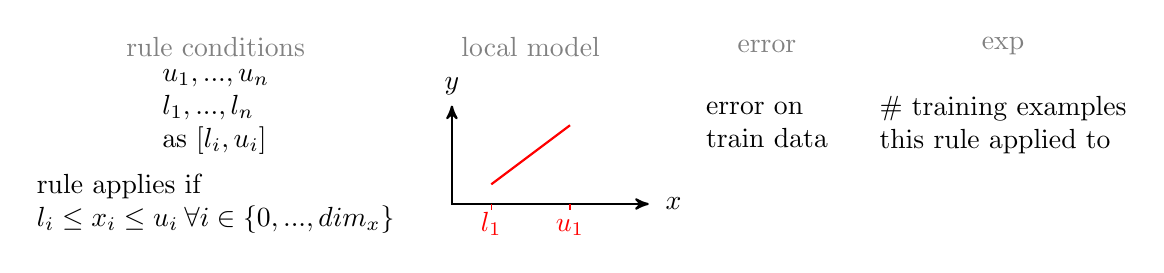
\begin{tikzpicture}[every node/.style={draw=none,minimum width=2cm,align=center}]
  
  \draw node[text=gray] (cond) {rule conditions};
  \draw node[below of=cond, align=left] (tcond) {$u_1,...,u_n$\\
    $l_1,...,l_n$\\
    as $[l_i,u_i]$\\};
  \draw node[below of=tcond, align=left] (expcond) {rule applies if\\
    $l_i \leq x_i \leq u_i \: \forall i \in \{0,...,dim_x\}$};
  
  \draw node[text=gray,right of=cond,xshift=3cm] (mod) {local model};
  \draw [<->,thick,scale=0.5] (6,-1.5) node (yaxis) [above] {$y$}
        |- (11,-4) node (xaxis) [right,xshift=-0.7cm] {$x$};
  \draw[red,thick,scale=0.5] (7,-3.5) coordinate (a) -- (9,-2) coordinate (b);
  \draw[dashed,scale=0.5] (xaxis -| a) node[text=red] at (7,-4.5) (l) {$l_1$};
  \draw[dashed,scale=0.5] (xaxis -| b) node[text=red] at (9,-4.6) (u) {$u_1$};
  \draw[dashed,red,scale=0.5] (l) ++ (0,0.35) to (7,-4);
  \draw[dashed,red,scale=0.5] (u) to (9,-4); 
      
  \draw node[text=gray,right of=mod,xshift=2cm] (error) {error};
  \draw node[below of=error,align=left] (terr) {error on\\ train data};
  
  \draw node[text=gray,right of=error,xshift=2cm] (exp) {exp};
  \draw node[below of=exp,align=left] (texp) {\# training examples\\ this rule applied to};
  

\end{tikzpicture}

\end{page}

\end{document}